%
%	Uyghur latex typesetting example
%	Anwar Mamat
%	anwarmamat@gmail.com
%

\documentclass[24]{article}

\usepackage{setspace}
\usepackage{multicol}
\usepackage{amsmath}
 \usepackage{verbatim}
\usepackage{algorithm}
\usepackage{algorithmic}
\usepackage{verse}
\usepackage{chemfig}
\renewcommand*\printatom[1]{\ensuremath{\mathsf{#1}}}
\usepackage{fontspec}
\usepackage{wrapfig}
%\usepackage{arabxetex}
\usepackage{polyglossia}


\setmainlanguage{english}
\setotherlanguage{arabic}

\newcommand\attrib[1]{\nopagebreak{\raggedleft\footnotesize #1\par}}
\newlength\lineindent
\newcommand*\setlineindent[1]{%
  \settowidth\lineindent{#1}%
  \addtolength\lineindent{-\vgap}%
  \addtolength\lineindent{-10pt}}
  
\renewcommand{\familydefault}{\sfdefault}



\newfontfamily\arabicfont[Script=Arabic,Scale=1.5]{UKIJ Tuz}

\begin{document}


\title{\textarabic{\LaTeX  تە ئۇيغۇرچە بەتنى قانداق ياسايمىز؟ }}
%\thanks{123456789}}
%\title{}
\author{
{\em } \\\textarabic{ئەنۋەر مەمەت \footnote{\textarabic{مەن بەت ياساشقا قىزىقىپ بۇنى ياساپ باقتىم.}}}\\
{\em anwar@temple.edu}\\
}

%\title{Real-Time Divisible Load Scheduling for Cluster Computing}

\date{}
\maketitle{}
\thispagestyle{empty}





\begin{Arabic}
\newfontfamily\arabicfont[Script=Arabic,Scale=1.5]{UKIJ Tuz}
\section{\textarabic{ جەدۋەل }}
\end{Arabic}
\newfontfamily\arabicfont[Script=Arabic,Scale=1]{UKIJ Basma}

\begin {table}[h]
\caption {\textarabic{بىزنىڭ ھۆنەرۋەنلىرىمىز}} \label{tab:people} 
\begin{center}
\begin{Arabic}
    \begin{tabular}{ | l | l | l | l |}
    \hline
   {ئىسمى ئاتىسى} & كەسپى & تېلفون &  يۇرتى{}  \\ \hline
    ئەمەت تۇرسۇن & ياغاچچى & 456-1234 & قەشقەر كوناشەھەر \\ \hline
    ھەسەن سىدىق & تۆمۈرچى & 325-4325 & غۇلجا دادامتۇ \\ \hline
    تۇرسۇن پالتاجى & سازچى & 281-4534 & خوتەن قارىقاش\\
    \hline
    
    \end{tabular}
    \end{Arabic}
\end{center}
\end{table}

\begin{Arabic}

%\RLmulticolcolumns
\newfontfamily\arabicfont[Script=Arabic,Scale=1.5]{UKIJ Tuz}
\section{\textarabic{كۆپ ستون }}
\begin{multicols}{3}
1. تاش چىراغ. باركۆل ناھىيىسىدىن مىلادىدىن ئىلگىرىكى دەۋرلەرگە تەۋە بىر خارابىلىكتىن بىر دانە تاش چىراغ تېپىلغان. بۇ چىراغنىڭ ئېگىزلىكى 31 سانتىمېتىر بولۇپ، چاسا تەگلىك شەكلىدە ياسالغان. چىراغنىڭ بىر يېنىغا مايمۇننىڭ شەكلى ئويۇلغان. 1972 – يىلى تۇرپان ئاستانە قەدىمكى قەبرىستانلىقىدىكى 177 – نومۇرلۇق قەبرىدىن بىر دانە ئىپتىدائىي تاش چىراغ قېزىۋېلىنغان. بۇ چىراغ خېلى بۇرۇنقى دەۋرلەردە ياسالغان، ئەمما تاڭ سۇلالىسى دەۋرىگە كەلگەندە جەسەت بىلەن قويۇلغان، دەپ پەرەز قىلىنغان. چىراغنىڭ ئېگىزلىكى 11.8سانتىمېتىر، ئۇزۇنلۇقى 12 سانتىمېتىر بولۇپ، ئۇ ھازىر ئاپتونوم رايونلۇق مۇزېيدا ساقلانماقتا.

2.ساپال {\huge{چىراغ}}. 1961 – يىلى مۇڭغۇلكۈرە ناھىيىسىدىكى شوتا قەدىمكى قەبرىستانلىقىنى ئارخېئولوگىيىلىك تەكشۈرۈشتە 7 – نومۇرلۇق قەبرىدىن بىر دانە ساپال چىراغ قېزىۋېلىنغان. بۇ چىراغنىڭ ئېغزى يايپاڭ، تېگى دۈگىلەك، ئومۇمىي ئېگىزلىكى 9.5 سانتىمېتىر. 1997 – يىلى خەنزۇچە نەشر قىلىنغان ‹‹شىنجاڭنىڭ مەدەنىيەت يادىكارلىقى – ئارخېئولوگىيە خىزمىتىدىكى يېڭى ھاسىلاتلار›› دېگەن كىتابقا كىرگۈزۈلگەن ‹‹1995 – يىلى تۇرپان يارغول قەدىمكى شەھىرى غەربىي غول قەبرىستانلىقىنى قىزىشتىن قىسقىچە دوكلات››تىكى مەلۇماتلارغا قارىغاندا، قەدىمكى تۇرپان خەلقى ساپال چىراغ ياساشتا ھەر خىل يېڭى تېخنىكا ۋە ھۈنەر – سەنئەتنى قوللىنىپ، چىراغلارنىڭ ياسىلىش شەكلى ۋە سۈپىتى جەھەتتە شۇ دەۋرلەرگە نىسبەتەن يېڭىلىق ياراتقان.
\end{multicols}
\end{Arabic}


\begin{Arabic}



\newfontfamily\arabicfont[Script=Arabic,Scale=1.5]{UKIJ Tuz}
\section{\textarabic{رەسىم قىستۇرۇش}}



3. لاي چىراغ. لايدا ياسالغان بۇنداق چىراغلار ئاساسەن تۇرپان ئاستانىدىكى مىلادىيە 4 – ئەسىردىن 8 – ئەسىرگىچە بولغان دەۋرگە تەۋە قەبرىلەردىن قېزىۋېلىنغان. ئۇلارنىڭ سانىمۇ خېلى كۆپ. مەسىلەن: تۇرپان ئاستانىدىكى 307 – نومۇرلۇق قەبرىدىن ئۈچ دانە، 327 – نومۇرلۇق قەبرىدىن 12 دانە لاي چىراغ قېزىۋېلىنغان. بۇ چىراغلار قولدا ياسالغان بولۇپ، شەكلى ئاددىي، ياسىلىشى بىر قەدەر قوپال.

\begin{wrapfigure}{r}{0.6\textwidth}
  \begin{center}
    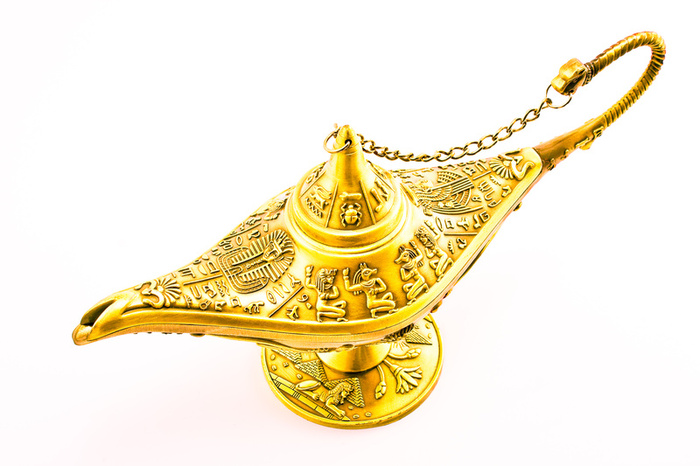
\includegraphics[width=0.58\textwidth]{lamp.jpg}
  \end{center}
  %\caption{چىراغ}
\end{wrapfigure}
4.ياغاچ چىراغ. دىيارىمىزدىكى ئارخېئولوگىيىلىك قېزىشلاردا ياغاچ چىراغ ناھايىتى ئاز بايقالغان. ئۇلارنىڭ دەۋرى مىلادى 5 – ئەسىردىن 9 – ئەسىرگىچەبولغان دەۋرلەرگە توغرا كېلىدۇ. بۇ چىراغلار ھازىر ئاپتونوم رايونلۇق مۇزېيدا ساقلىنىۋاتىدۇ.

5. مىس چىراغ. 1959 – يىلى مارالبېشى ناھىيىسىنىڭ توققۇزساراي خارابىسىدىن ناھايىتى نەپىس قۇيۇلغان، ئۆزگىچە ئالاھىدىلىككە ئىگە، ئېگىزلىكى 7.3 سانتىمېتىر كېلىدىغان بىر دانە مىس چىراغ تېپىلغان. مۇشۇ خارابىدىن بايقالغان يادىكارلىقلارغا ئاساسەن، ئۇ مىلادىيىنىڭ ئالدى – كەينىدىكى دەۋرلەرگە مەنسۇپ دەپ قارالماقتا.

6.قاشتېشى چىراغ. ئۈچ پىلىكلىك بۇنداق چىراغ قەشقەر شەھىرىدىن تېپىلغان بولۇپ، ئېگىزلىكى 12 سانتىمېتىر، كەڭلىكى 23 سانتىمېتىر، ئۈچ پىلىكلىك بۇ چىراغ ئاق قاشتېشىدىن ئويۇلغان بولۇپ، خالىغان جايغا تۈز قويۇشقىمۇ، ئېسىپ قويۇشقىمۇ بولىدۇ. ئىشلەتكەندە ئۈچ پىلىكىنى تەڭلا يورۇتۇشقىمۇ بولىدۇ.

ئۇزاق تارىختىن بۇيان ئەجدادلىرىمىز تەرىپىدىن ياغ چىراغ، پىلىك چىراغ، جىنچىراغ، كىرسىن چىراغ دەپ ئىشلىتىلىپ كەلگەن بۇ چىراغلار تاش قوراللار دەۋرىدە تاشتىن ۋە ياغاچتىن، برونزا(كۆك مىس) دەۋرىدە مىس ۋە قاشتېشى قاتارلىقلاردىن ياسالغان. بولۇپمۇ ئەجدادلىرىمىز مېتالچىلىق دەۋرىگە قەدەم قويغاندا، مىس، تۆمۈر، چويۇن، پولات، قەلەي قاتارلىقلاردىن كۆركەم، چىرايلىق، سىپتا چىراغلار ياسىلىپ پايدىلىنىلغان. شۇڭا، ئەجدادلىرىمىزنىڭ چىراغ مەدەنىيىتى ھەققىدە تېخىمۇ ئەتراپلىق ئىزدىنىشىمىزگە توغرا كېلىدۇ.
\end{Arabic}

\newfontfamily\arabicfont[Script=Arabic,Scale=1]{UKIJ Basma}
\begin{Arabic}
%\RLmulticolcolumns
\newfontfamily\arabicfont[Script=Arabic,Scale=1.5]{UKIJ Tuz}
\section{\textarabic{شېئىر}}
\end{Arabic}




\newfontfamily\arabicfont[Script=Arabic,Scale=1.5]{UKIJ Esliye}
\begin{Arabic}
\begin{center}
شەيتان

شەيخ سەئىدى
\end{center}

\hspace {1in}
    ئەل ھەققىنى  يەيتى دائىم بىر ئەبلەخ
 
 \hspace {1in}
ئەمما تىللاپ تۇرار ئىدى شەيتاننى

 \hspace {1in}
دىدى بىر كۈن شەيتان ئاڭا دۇچ كىلىپ:

 \hspace {1in}
ئۇچراتمىدىم سەندەك رەزىل ئىنساننى.

 \hspace {1in}
كۆڭۈلدىغۇ خېلى يېقىن تۇققان بىز،

\hspace {1in}
نىمە بۇنداق تىللاپ يۈردۈڭ تۇتامسىز؟

\end{Arabic}



\newfontfamily\arabicfont[Script=Arabic,Scale=1]{UKIJ Basma}
\begin{Arabic}
%\RLmulticolcolumns
\newfontfamily\arabicfont[Script=Arabic,Scale=1.5]{UKIJ Tuz}
\section{\textarabic{تىزىملىك}}
\end{Arabic}

\begin{Arabic}
\begin{itemize}
\item ئائىلە ۋە دوستلار خىزمەتتىن مۇھىم.
\item داۋامىلىق راستچىل بولۇڭ. يالغاننى ئەستە ساقلىماق بەك تەس.
\item ئۆزى ياخشى كۆرمەيدىغان ئىشنى قىلىشقا ھايات بەك قىسقا كىلىدۇ.
\item ئۆزى قىلالمايمەن دىيىشتىن بۇرۇن، باشقىلارنى ئۇ ئىشنى قىلالايدۇ دەپ ئويلاڭ
\end{itemize}
\end{Arabic}


\newfontfamily\arabicfont[Script=Arabic,Scale=1]{UKIJ Basma}
\begin{Arabic}
%\RLmulticolcolumns
\newfontfamily\arabicfont[Script=Arabic,Scale=1.5]{UKIJ Tuz}
\section{\textarabic{ماتېماتىكا}}
\end{Arabic}
\begin{align}
    E &= mc^2              \vspace{1.3in}  \hfill \mbox{ \textarabic{ئېينىشتىين}}              \\
    m &= \frac{m_0}{\sqrt{1-\frac{v^2}{c^2}}}    
  \end{align}
\begin{align*}
 &\vdots\\
 &=12+7 \int_0^2
  \left(
    -\frac{1}{4}\left(e^{-4t_1}+e^{4t_1-8}\right)
  \right)\,dt_1\displaybreak[3]\\
 &= 12-\frac{7}{4}\int_0^2 \left( e^{-4t_1}+e^{4t_1-8} \right)\,dt_1\\
 &\vdots %
\end{align*}

\begin{equation}
A_{m,n} =
 \begin{pmatrix}
  a_{1,1} & a_{1,2} & \cdots & a_{1,n} \\
  a_{2,1} & a_{2,2} & \cdots & a_{2,n} \\
  \vdots  & \vdots  & \ddots & \vdots  \\
  a_{m,1} & a_{m,2} & \cdots & a_{m,n}
 \end{pmatrix}
\end{equation}


\begin{equation}
\frac{\sum_{n > 0} z^n} 1≤k≤n(1−qk) {\prod_{1\leq k\leq n} (1-q^k)}
\end{equation}

\noindent
\begin{Arabic}
\newfontfamily\arabicfont[Script=Arabic,Scale=1.5]{UKIJ Tuz}
\section{\textarabic{خىمىيە}}
\end{Arabic}


\setcrambond{2pt}{}{}
\chemfig{
  HO-[2,.5,2]?<[7,.7](-[2,.5]OH)-[,,,,line width=2.4pt](-[6,.5]OH)>[1,.7]
    (-[:-65,.7]O-[:65,.7]?[b](-[2,.7]CH_2OH)<[:-60,.707](-[6,.5]OH)
      -[,,,,line width=2.4pt](-[2,.5,,2]HO)>[:60,.707](-[6,.5]CH_2OH)-[:162,.9]O?[b])
  -[3,.7]O-[4]?(-[2,.3]-[3,.5]HO)}




\setatomsep{2em}
\chemfig{
  H_3C-[:72]{\color{blue}N}
    *5(-
      *6(-(={\color{red}O})-{\color{blue}N}(-CH_3)-(={\color{red}O})-{\color{blue}N}(-CH_3)-=)
    --{\color{blue}N}=-)}

\begin{Arabic}
%\RLmulticolcolumns
\newfontfamily\arabicfont[Script=Arabic,Scale=1.5]{UKIJ Tuz}
\section{\textarabic{كومپيوتېر پىروگىراممىسى}}
\end{Arabic}
\begin{algorithm}
\caption{\textarabic{پىروگىرامما}($\tau(A,\sigma,D)$,\textarabic{مىقدارى} )}
\label{uyghur-alg}
\begin{algorithmic}[1]
\STATE \textarabic{ئاۋال ھەر بىر نوقتىنىڭ ھالىتىنى تەكشۈرىدۇ.}
\IF{($\tau.(A + D) \leq P_0$.AvailableTime + $\tau.\sigma C_{ms}$)} \RETURN {\bf false} \ENDIF
\STATE $\tau_p$ = getPredecessor($\tau$)  \label{getPredecessor2}

\STATE $\tau_s$ = getSuccessor($\tau$) \label{getSuccessor2}
\STATE $\tau.{\cal E}=  {\cal E}(\tau.\sigma,N)$

\IF{($\tau_s \neq$ null \&\& $\tau.{\cal E}>\tau_s.slack_{min}$)}
\RETURN {\bf false}
\ENDIF


\IF{($\tau_p == $ null)}
\STATE $\tau.S = \tau.A$
\ELSE
\STATE  $\tau.S = \tau_p.C$
\IF{(TWQ == $\emptyset$)}
\STATE adjust($\tau$)
\ENDIF

\STATE $\tau.S= max(\tau.S, \tau.A)$
\ENDIF

\IF{$\tau.(A+D-S)<\tau.{\cal E}$}

\RETURN {\bf false}
\ELSE
\STATE $\tau._{slack} = \tau.(A + D - S - {\cal E})$
\STATE $\tau.C = \tau.(S + {\cal E})$
\STATE TWQ.insert($\tau$)
\STATE updateSlacks($\tau$, TWQ)
\FOR{($\tau_i\in$ TWQ \&\& $\tau_i.(A+D)>\tau.(A+D)$)}
\STATE $\tau_i.C +=\tau.{\cal E}$
\ENDFOR

\RETURN {\bf true}

\ENDIF

\end{algorithmic}
\end{algorithm}


\begin{algorithm}
\caption{\textarabic{ئۇيغۇرچە پىروگىرامما}}
\label{uyghur-alg}
\begin{algorithmic}
\IF{ \textarabic{دادا ياخشى بولسا}}
\IF {\textarabic{ئانا ياخشى بولسا}}
\STATE \textarabic{بالا ياخشى بولىدۇ}
\ENDIF
\ENDIF
\end{algorithmic}
\end{algorithm}



\end{document}